% (c) Noah Jutz
% All rights reserved.

\documentclass{article}
\usepackage[utf8]{inputenc}
\usepackage[german]{babel}
\usepackage{graphicx}
\usepackage{float}
\usepackage{wrapfig,lipsum,booktabs}

\usepackage{biblatex,csquotes}
\addbibresource{main.bib}

\graphicspath{ {./images/} }

\title{Entwicklung eines IR-Spektrometers}
\author{Noah Jutz}
\date{}

\begin{document}

\maketitle
\tableofcontents

\newpage
\section{Einführung}
% 1.1 Spektroskopie
% 1.1.1 Was ist es generell?
Spektroskopie ist ein Überbegriff für analytische Verfahren, die eine Strahlung zerlegen. Die gemessene Strahlungsintensität liefert ausschlaggebende Information über die molekulare Zusammensetzung einer Substanz.

% 1.1.2 Was ist Prisma-Spektroskop?
Als Beispiel zerlegt ein Prismenspektrometer eine Strahlquelle mit einem Prisma. Das resultierende Spektrum offenbart bei Sonnenlicht alle Wellenlängen bzw. Farben im sichtbaren Wellenlängenbereich (ca. 400nm-700nm) \cite{TODO}. Auch zu erkennen sind dunkle Linien bei bestimmten Wellenlängen (Abb. \ref{fig:fraunhofer-linien}). Diese werden als Absorptionslinien oder \textbf{Fraunhofer'sche Linien} bezeichnet.

\begin{figure}[ht]
    \centering
    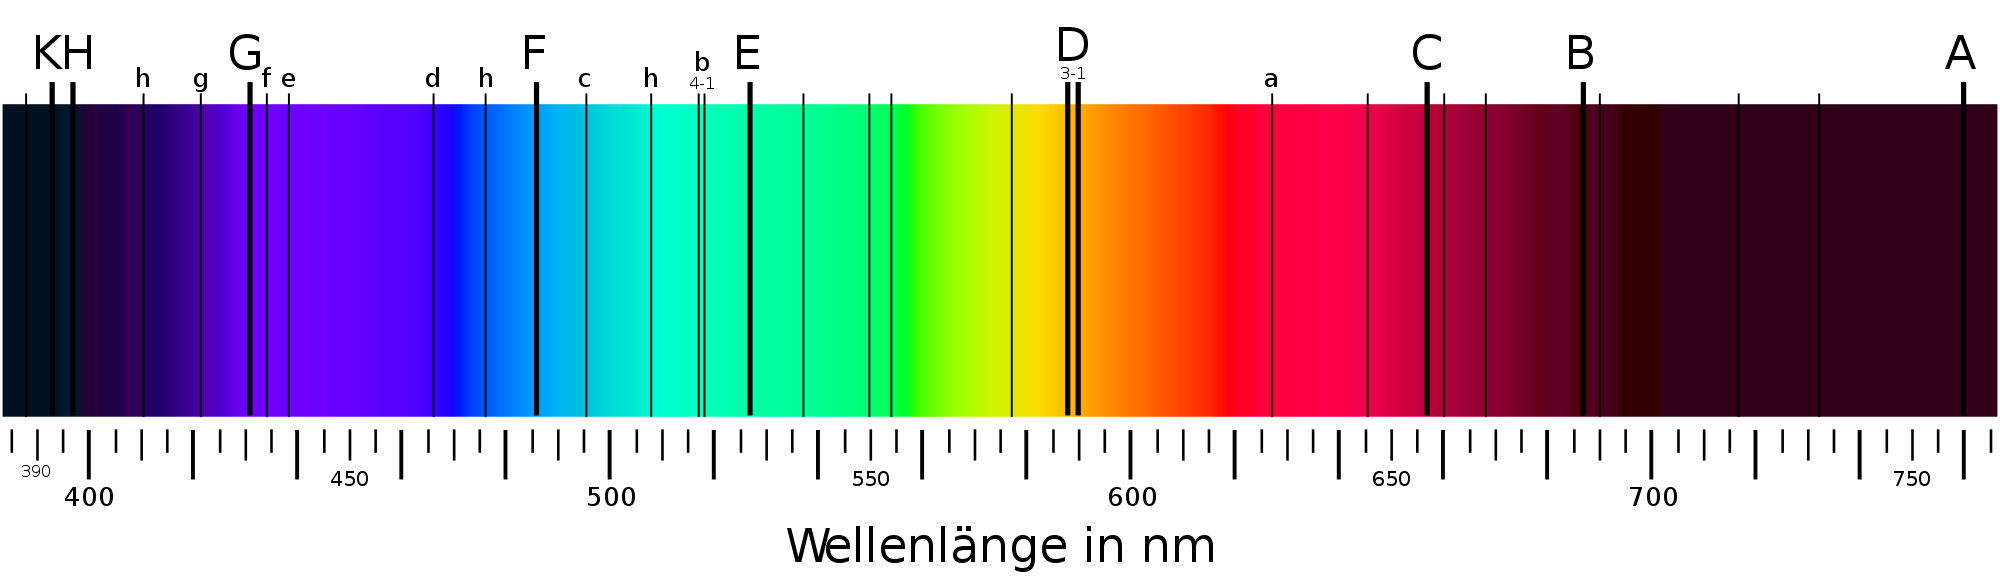
\includegraphics[width=0.65\textwidth]{fraunhofer_linien.png}
    \caption{Fraunhofer'sche Linien im Sonnenlichtspektrum \cite{TODO}}
    \label{fig:fraunhofer-linien}
\end{figure}

% 1.2 Fraunhoferlinien
% 1.2.1 Entdeckung Fraunhofer
Joseph Fraunhofer entdeckte und dokumentierte 1814 sorgfältig über 570 dieser Linien \cite{TODO}. Mit seinen Ergebnissen konnte er hochwertige astronomische Fernrohre herstellen.

% 1.2.2 Entdeckung Bunsen, Kirchhoff
1859 führten Gustav Robert Kirchhoff und Robert Bunsen ein Experiment durch, bei dem eine Assoziazion zwischen chemischen Elementen und den Fraunhofer'schen Linien beobachtet wurde \cite{TODO}. Daraus folgt, dass die Absorptionslinien des Sonnenspektrums, welche Fraunhofer analysierte, die Absorptionseigenschaften dieser Elemente reflektieren.

% 1.3 IR-Spektroskopie
% 1.3.1 Was ist es?
Die IR-Spektroskopie ist eine Methode der Molekülspektroskopie, welche sich mit den zwischenmolekularen Kräften in Molekülstrukturen beschäftigt. Bei der Infrarotspektroskopie werden Wellen im Infrarotbereich (ca. 800nm-1mm) \cite{TODO} zerlegt.

% 1.3.2 Vgl. Fraunhofer
Genau wie bei Fraunhofers Lichtspektrometer dient die Infrarotspektroskopie dem Nachweis chemischer Stoffe. Während das Lichtspektrometer die chemische Zusammensetzung der Sterne durch die Absorption am sichtbaren Licht der dortigen Elemente nachweist, kann das Infrarotlicht eines IR-Spektrometers Schwingungen in bestimmten chemischen Gruppen anregen \cite{TODO}, und somit in gewissen Wellenlängenbereichen Absorptionen herbeirufen.

% 1.3.3 Methoden: FTIR, Laser, Raman, ATR, etc.
Zu den arten der IR-Spektroskopie gehören u. A. FTIR-, Raman-, und ATR-Spektroskopie.

\newpage
\section{Theoretische Grundlagen}

% 2. Übergang
Um die Funktionsweise eines IR-Spektrometers zu verstehen, müssen zunächst folgende Theoretische Grundlagen aufgeklärt werden.

\subsection{Interferenz}

% 2.1.1 Was ist es?
Der Begriff der Interferenz beschreibt das Verhalten von Wellen bei Überlagerungen.

% 2.1.2 Grundsatz
Grundsätzlich heißt es in der Physik, dass bei der Überlagerung von Wellen ihre Amplituden addiert werden. Das heißt, dass z.B. das Aufeinanderstoßen zwei gleich hoher Wellen zu einer verdoppelung der Amplitude führt.

\begin{wrapfigure}{r}{0.3\textwidth}
    \centering
    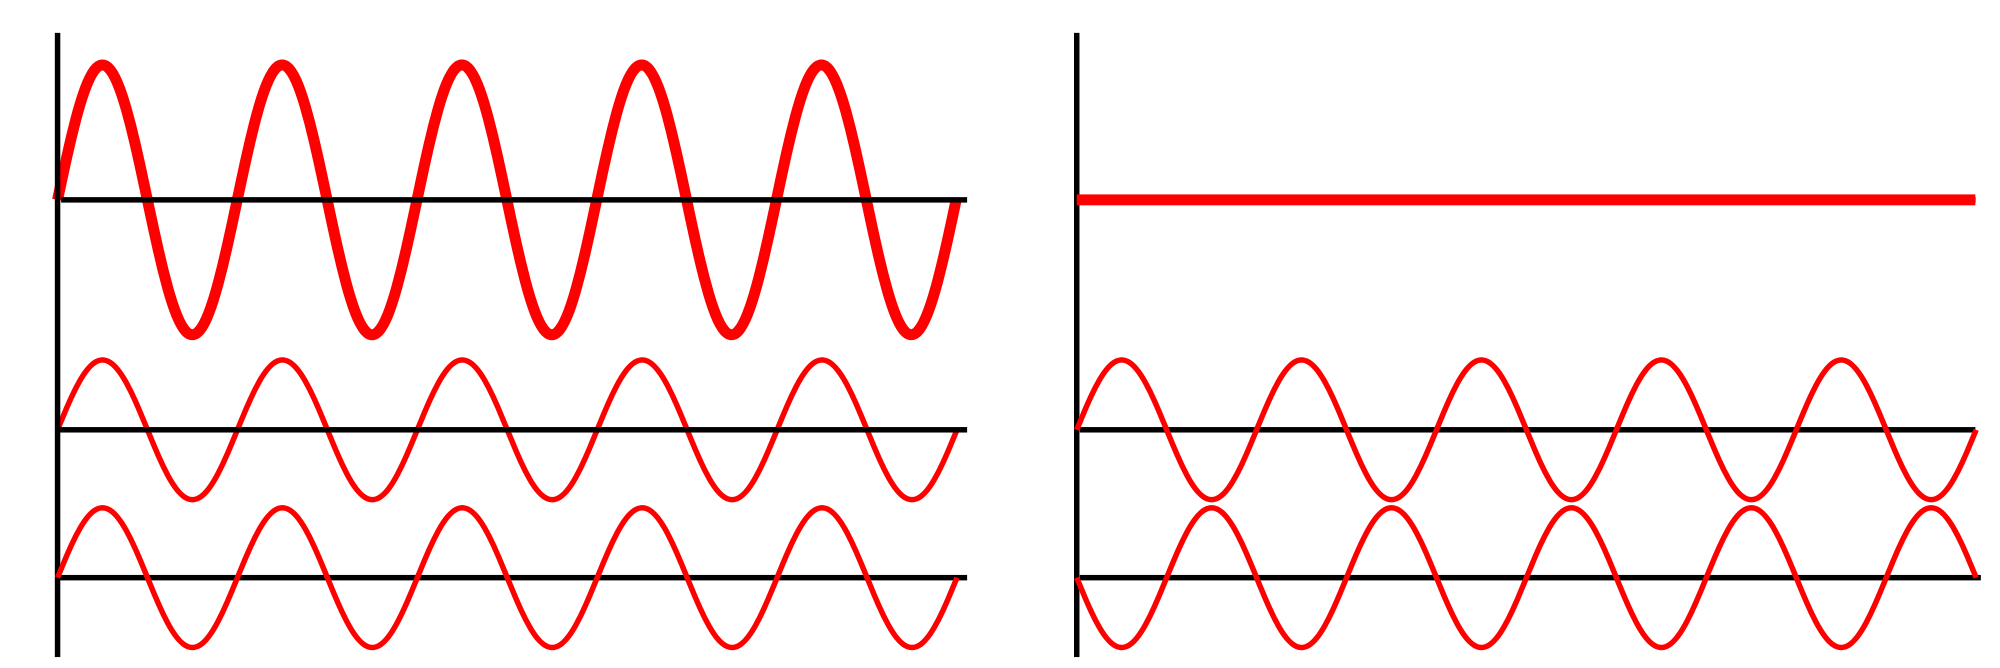
\includegraphics[width=0.3\textwidth]{interferenz.png}
    \caption{Konstruktive (links) und Destruktive Interferenz (rechts) \cite{TODO}}
    \label{fig:interferenz}
\end{wrapfigure}
% 2.1.3 Konstruktiv
Man spricht hier also von Konstruktiver Interferenz - wenn zwei Wellen aufeinander treffen, bei welchen die Hoch- bzw. Tiefpunkte überlagern. Voraussetzung ist, dass der Gangunterschied zwei koharänter Wellen das Vielfache ihrer Wellenlänge $\lambda$ beträgt \cite{TODO}.
\begin{equation}
    \Delta s = m \lambda
\end{equation}
Das heißt, dass Wellenhochpunkt auf Wellenhochpunkt und Wellentiefpunkt auf Wellentiefpunkt treffen. Daraus folgt, dass die summierte resultierende Welle eine höhere Amplitude hat. (Abb. \ref{fig:interferenz})

% 2.1.4 Destruktiv
Im Gegenzug heißt destruktive Interferenz, dass ein Wellenhochpunkt auf einen Tiefpunkt zukommt, und eine Welle mit kleinerer Amplitude herauskommt. Dabei kann es auch zur kompletten Auslöschung der Welle kommen. Vorraussetzung ist, dass der Gangunterschied $\Delta s$ ein Vielfaches der Wellenlänge $\lambda$ ist und um $\frac{1}{2} \lambda$ verschoben ist \cite{TODO}.
\begin{equation}
    \Delta s = (m - \frac{1}{2}) \lambda
\end{equation}
Somit treffen Hochpunkte auf Tiefpunkte und umgekehrt. (Abb. \ref{fig:interferenz})

% 2.1.5 Mathematische Darstellung
Die Ausbreitung der Welle wird als Mathematische Formel normalerweise als $f(x, t)$ beschrieben, wo $x$ die Position der Welle und $t$ der Zeitpunkt der Ausbreitung ist. Somit kann die Überlagerung mehrerer Wellen $f_i(x, t)$ am Punkt $x_0$ beim Zeitpunkt $t$ als Summe der einzelnen Wellen betrachtet werden \cite{TODO}.
\begin{equation}
    f_{ges}(x_0, t) = \sum_{i}f_i(x_0, t)
\end{equation}

% 2.1.6 Warum Grundlage?
Interferenz ist bei der IR-Spektroskopie ein relevanter Begriff, weil das Infrarotlicht nach dem durchdringen einer Substanz am Detektor durch die Interferenz der IR-Wellen ein bestimmtes Wellenmuster aufweist, welches am Detektor ausgemessen und zum Spektrum ausgewertet werden kann. 

\newpage
\subsection{Doppelspaltexperiment}

% 2.2.1 Was ist es?
Das klassische Doppelspaltexperiment weist das Wellenartige Verhalten von Licht durch die Interferenz der Wellen nach.
% 2.2.2 Geschichte / Entdeckung
Das Experiment wurde erstmals 1801 von Thomas Young durchgeführt \cite{TODO}.

\begin{wrapfigure}{r}{0.3\textwidth}
    \centering
    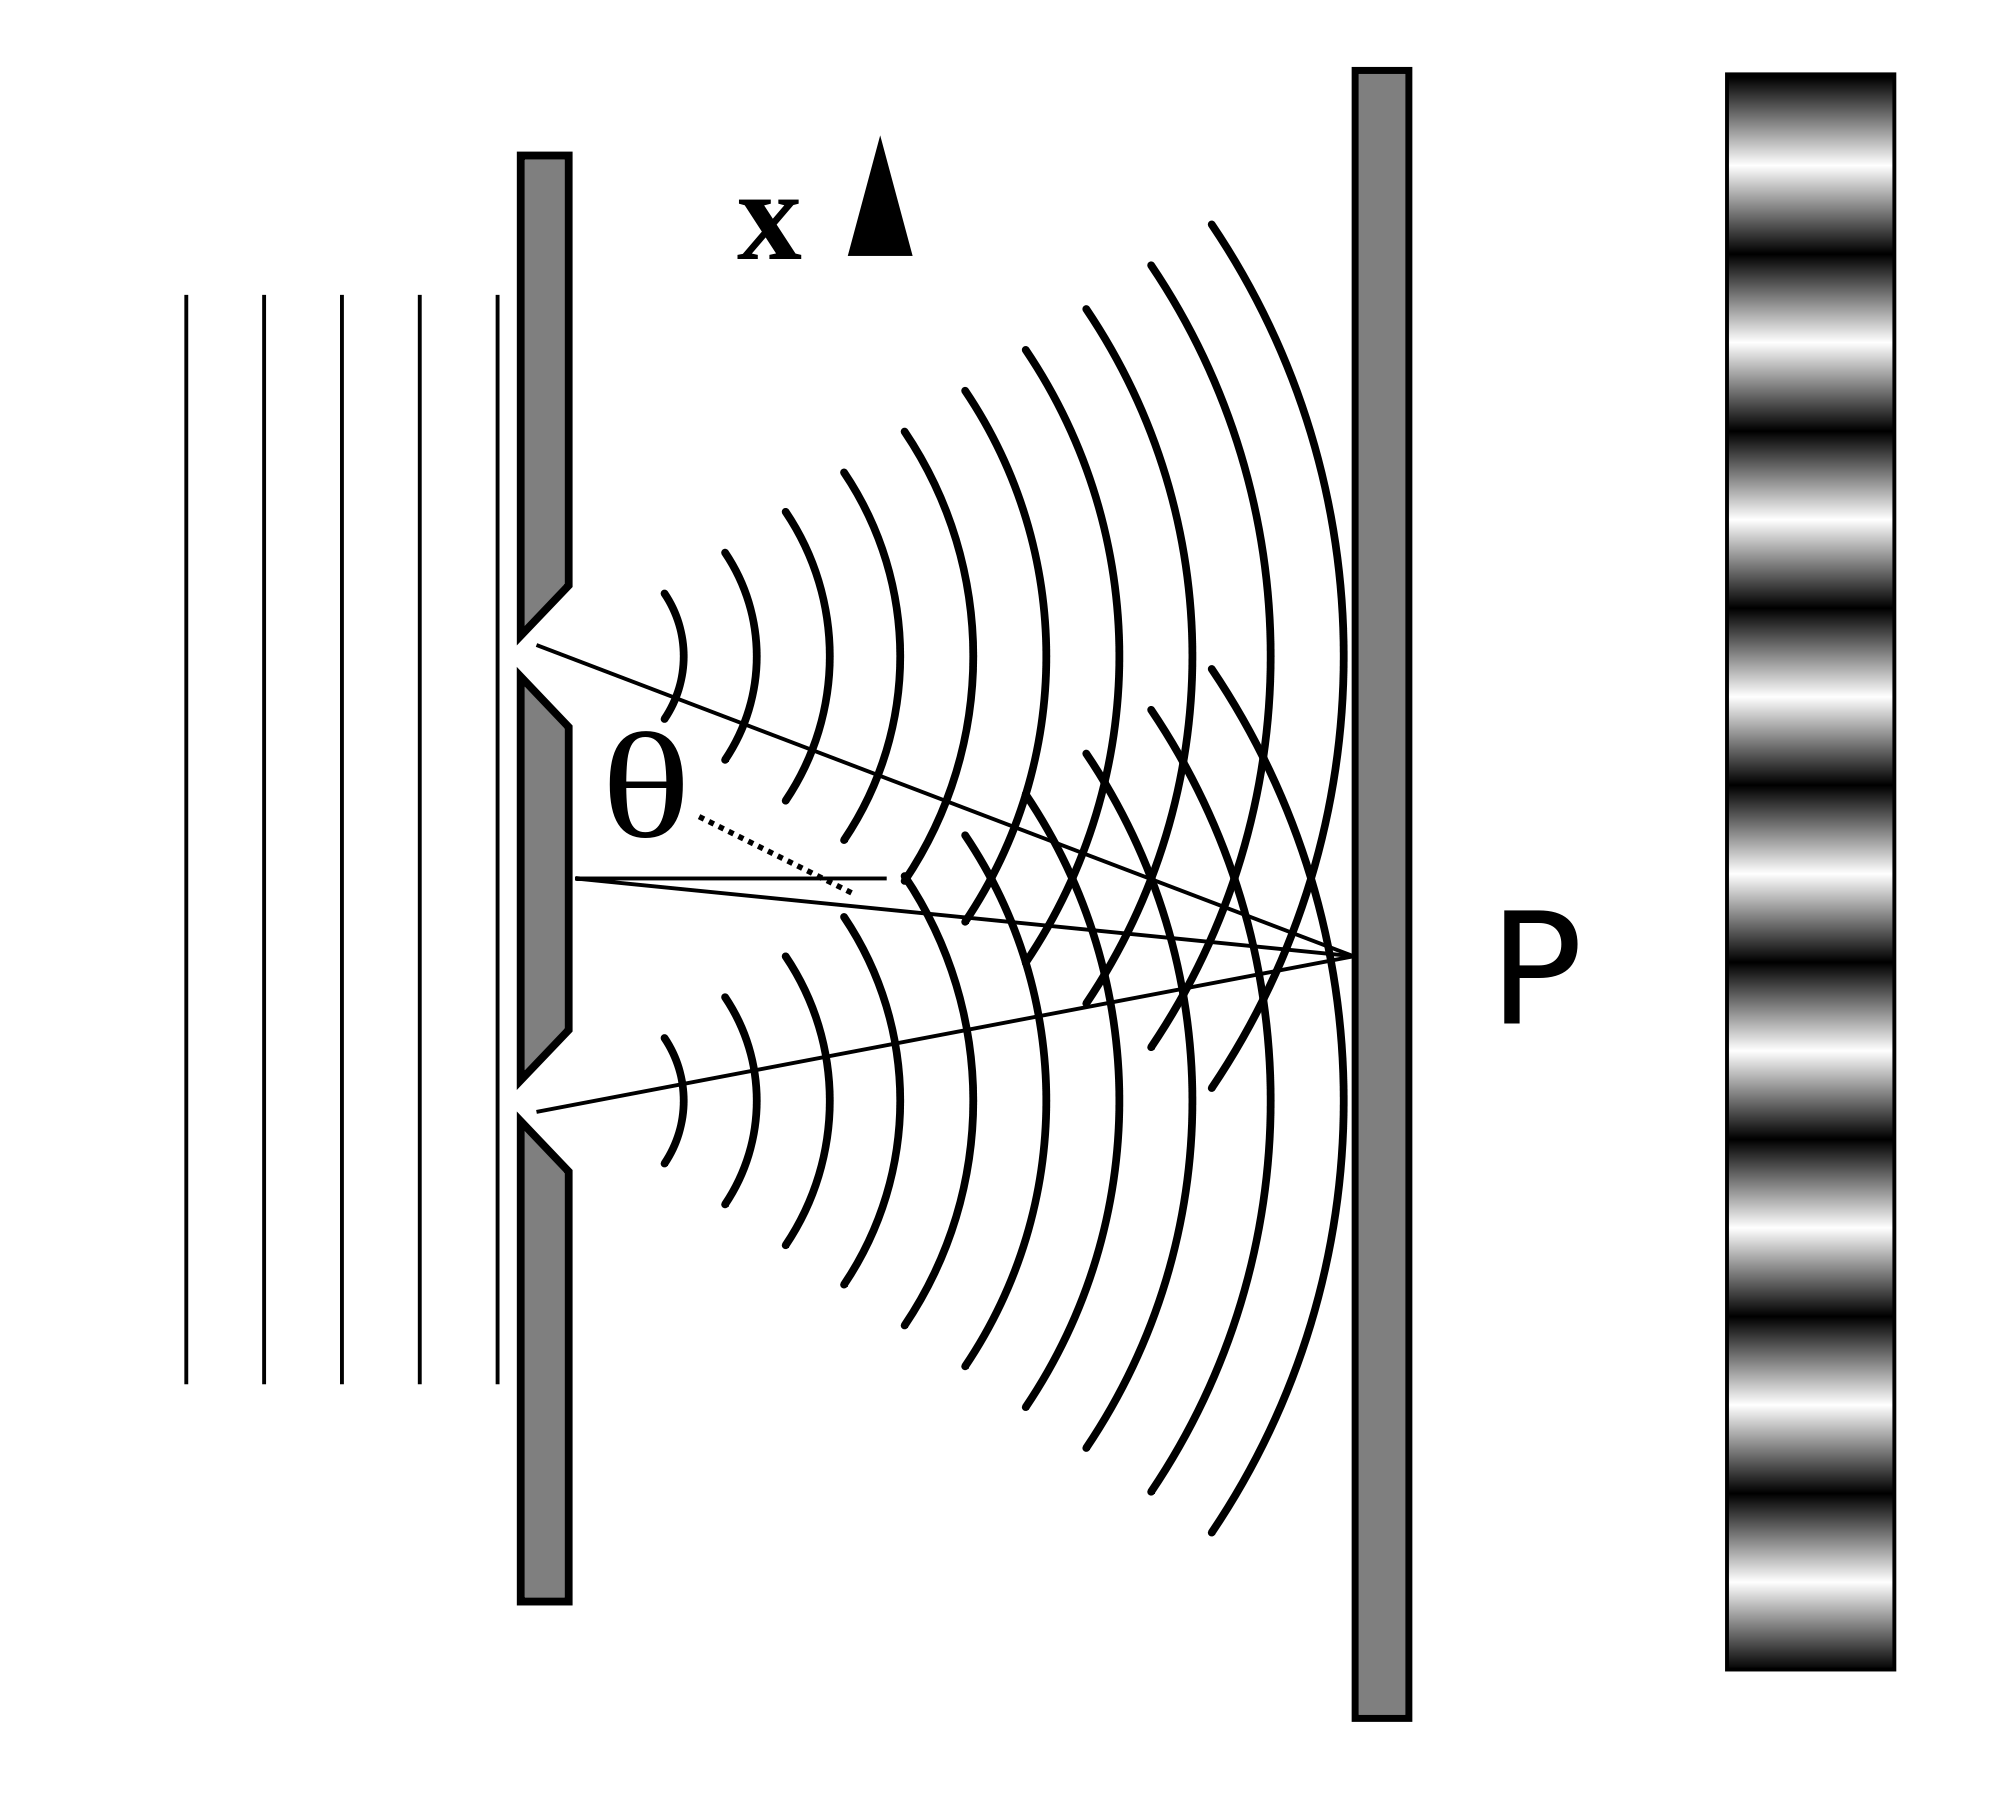
\includegraphics[width=0.3\textwidth]{doppelspalt.png}
    \caption{Doppelspaltexperiment \cite{TODO}}
    \label{fig:doppelspalt}
\end{wrapfigure}
% 2.2.3 Aufbau
Der Aufbau ist wie folgt (Abb. \ref{fig:doppelspalt}): Eine Lichtquelle (links), welche auf eine Wand mit zwei Spalten zukommt. Daneben eine geschlossene Wand, auf der das Licht aufkommt (rechts).

% 2.2._ Warum Grundlage?
% ...

\newpage
\subsection{Absorption}

% Warum Grundlage?

\section{IR-Spektrometer}

% Übergang

\subsection{Komponenten}

\subsubsection{Strahlquelle}

% λ × T = b
% Lötkolben

\subsubsection{Abbildende Optik}

% Spiegel

\subsubsection{Gitter}

% 600 Linien / mm
% Leypold
% Reflexionsgitter

\section{Versuch und Ergebnisse}

% b = k × λ ÷ sin(α)
%   α = 30°; λ = 530nm
%   -> b = 1500nm

\subsection{Versuchsaufbau}

% Bilder:
%   - loetkolben
%   - hg-lampe
%   - spiegel
%   - sensor
%   - gitter

\subsection{Ergebnisse}

% Diagramme
% Fehler

\section{Arduino} % Später

\subsection{Motorsteuerung}

\subsection{Signalerfassung}

\newpage
\printbibliography[heading=bibintoc]

\end{document}